% Préambule commun des schémas TikZ (compilés séparément par construire_figures.py)
\documentclass[tikz,border=3pt]{standalone}
\usepackage[T1]{fontenc}
\usepackage[utf8]{inputenc}
\usepackage{lmodern}
\usepackage{amsmath,amssymb}
\usepackage{bm}
\usepackage[american,siunitx,straightvoltages]{circuitikz}
\usetikzlibrary{arrows.meta,positioning,calc,decorations.pathmorphing,
  decorations.markings,decorations.pathreplacing,patterns,shapes.geometric,
  shapes.misc,shapes.multipart,fit,backgrounds,3d,intersections,matrix}

\ctikzset{bipoles/length=1.1cm, amplifiers/scale=0.85, tripoles/op amp/width=1.4}

\tikzset{
  >={Latex[length=2mm,width=1.4mm]},
  every picture/.style={line width=0.6pt, font=\small},
  % schémas-blocs
  bloc/.style={draw, minimum width=1.5cm, minimum height=0.9cm, align=center,
               inner sep=3pt, fill=white},
  somme/.style={draw, circle, minimum size=4.5mm, inner sep=0pt, fill=white,
                path picture={\draw (path picture bounding box.north west)
                  -- (path picture bounding box.south east)
                  (path picture bounding box.north east)
                  -- (path picture bounding box.south west);}},
  gain/.style={draw, isosceles triangle, isosceles triangle apex angle=60,
               minimum size=8mm, inner sep=1pt, fill=white},
  bruit/.style={draw, circle, minimum size=4.5mm, inner sep=0pt, fill=white,
                path picture={\node at (path picture bounding box.center)
                  {\scriptsize$\ast$};}},
  cadre/.style={draw, dashed, rounded corners=1pt},
  cadrept/.style={draw, dash dot, rounded corners=1pt},
  fleche/.style={->},
  % mécanique
  bati/.style={pattern=north east lines, draw=none},
  ressort/.style={decorate, decoration={coil, aspect=0.4, segment length=2.2mm,
                  amplitude=2mm, pre length=2mm, post length=2mm}},
  zigzag/.style={decorate, decoration={zigzag, segment length=2mm,
                  amplitude=1.6mm, pre length=2mm, post length=2mm}},
  pivot/.style={draw, circle, fill=white, minimum size=2.2mm, inner sep=0pt},
  masse/.style={draw, fill=gray!25, minimum width=1.4cm, minimum height=0.8cm},
  cote/.style={<->, line width=0.4pt},
  axe/.style={->, line width=0.6pt},
  trait mixte/.style={dash dot, line width=0.4pt},
}

% Encastrement / bâti hachuré : \bati{(x1,y1)}{(x2,y2)} trace une ligne et ses hachures dessous
\newcommand{\bati}[3][0.18]{%
  \fill[pattern=north east lines] #2 rectangle ($#3+(0,-#1)$);
  \draw[line width=0.8pt] #2 -- #3;}

% Transducteur (deux cercles entrelacés) : \pic (t) at (x,y) {transducteur};  -> (t-o) entrée, (t-e) sortie
\tikzset{
  transducteur/.pic={\draw (-0.13,0) circle (0.24); \draw (0.13,0) circle (0.24);
    \coordinate (-o) at (-0.37,0); \coordinate (-e) at (0.37,0);
    \coordinate (-n) at (0,0.24); \coordinate (-s) at (0,-0.24);},
  bobine/.style={decorate, decoration={coil, aspect=0.7, segment length=1.4mm,
                 amplitude=1.6mm, pre length=1mm, post length=1mm}},
  sourcebruit/.style={draw, circle, minimum size=5mm, inner sep=0pt, fill=white,
                 label={[inner sep=0pt]center:$\ast$}},
  sourcecourant/.style={draw, circle, minimum size=5mm, inner sep=0pt, fill=white,
                 label={[inner sep=0pt]center:$\circledast$}},
}

% Composants compacts (pour les petits boîtiers des schémas-blocs)
\newcommand{\resistance}[2]{% de #1 à #2 (quelconque)
  \draw #1 -- ($#1!0.22!#2$) ($#1!0.78!#2$) -- #2;
  \draw[decorate, decoration={zigzag, segment length=1.5mm, amplitude=1.1mm}]
    ($#1!0.22!#2$) -- ($#1!0.78!#2$);}
\newcommand{\condensateur}[2]{% horizontal de #1 à #2
  \draw #1 -- ($($#1!0.5!#2$)+(-0.05,0)$) ($($#1!0.5!#2$)+(0.05,0)$) -- #2;
  \draw[line width=1pt] ($($#1!0.5!#2$)+(-0.05,0.14)$) -- ($($#1!0.5!#2$)+(-0.05,-0.14)$)
                        ($($#1!0.5!#2$)+(0.05,0.14)$) -- ($($#1!0.5!#2$)+(0.05,-0.14)$);}
% R // C horizontal : \RparC{(x,y)}{longueur}{écart}  (centre, longueur totale, écart vertical)
\newcommand{\RparC}[3]{%
  \coordinate (rcA) at ($#1+(-#2/2,0)$); \coordinate (rcB) at ($#1+(#2/2,0)$);
  \draw (rcA) -- ++(0.15,0) coordinate (rcA1) (rcB) -- ++(-0.15,0) coordinate (rcB1);
  \draw (rcA1) -- ++(0,#3/2) (rcA1) -- ++(0,-#3/2) (rcB1) -- ++(0,#3/2) (rcB1) -- ++(0,-#3/2);
  \resistance{($(rcA1)+(0,#3/2)$)}{($(rcB1)+(0,#3/2)$)}
  \condensateur{($(rcA1)+(0,-#3/2)$)}{($(rcB1)+(0,-#3/2)$)}}

\begin{document}
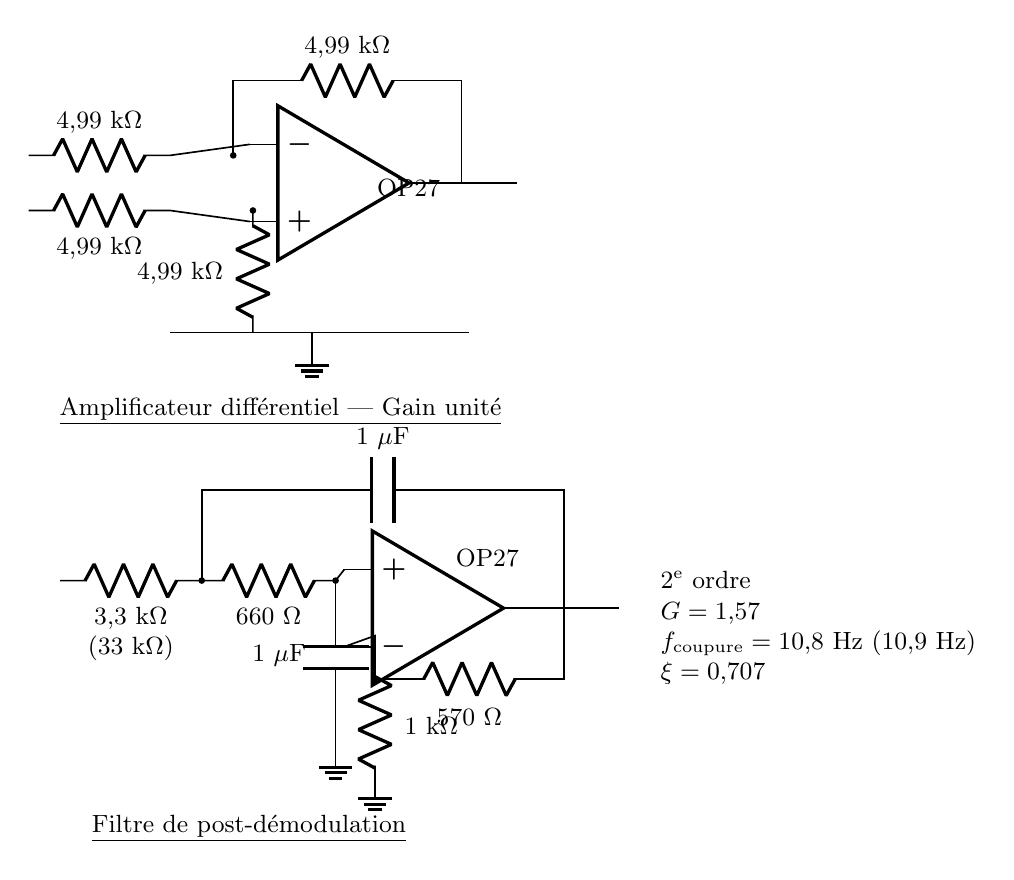
\begin{tikzpicture}[font=\small]
  % ---- amplificateur différentiel ----
  \begin{scope}
    \draw (3.4,0) node[op amp] (a) {};
    \node[right] at (a.east) {};
    \node[above right] at (3.7,-0.3) {OP27};
    \draw (-0.6,0.35) to[R, l=4{,}99 k$\Omega$] (1.2,0.35) -- (a.-);
    \draw (-0.6,-0.35) to[R, l_=4{,}99 k$\Omega$] (1.2,-0.35) -- (a.+);
    \fill (2.0,0.35) circle (1.2pt) (2.25,-0.35) circle (1.2pt);
    \draw (2.0,0.35) -- (2.0,1.3) to[R, l=4{,}99 k$\Omega$] (4.9,1.3) -- (4.9,0);
    \draw (a.out) -- (5.6,0);
    \draw (2.25,-0.35) to[R] (2.25,-1.9); \node[left] at (2.0,-1.15) {4{,}99 k$\Omega$};
    \draw (1.2,-1.9) -- (5.0,-1.9); \draw (3.0,-1.9) node[ground] {};
    \node[below] at (2.6,-2.6) {\underline{Amplificateur différentiel — Gain unité}};
  \end{scope}
  % ---- filtre de post-démodulation ----
  \begin{scope}[shift={(0,-5.4)}]
    \draw (4.6,0) node[op amp, noinv input up] (b) {};
    \node[above right] at (4.7,0.4) {OP27};
    \draw (-0.2,0.35) to[R, l_={\begin{tabular}{c}3{,}3 k$\Omega$\\(33 k$\Omega$)\end{tabular}}] (1.6,0.35);
    \fill (1.6,0.35) circle (1.2pt);
    \draw (1.6,0.35) to[R, l={(6{,}6 k$\Omega$)}, l_=660~$\Omega$] (3.3,0.35) -- (b.+);
    \fill (3.3,0.35) circle (1.2pt);
    \draw (3.3,0.35) to[C] (3.3,-1.6) node[ground] {}; \node[left] at (3.05,-0.6) {1 $\mu$F};
    \draw (1.6,0.35) -- (1.6,1.5) to[C, l=1 $\mu$F] (6.2,1.5) -- (6.2,0);
    \draw (b.out) -- (6.9,0);
    \draw (b.-) -- (3.8,-0.35) -- (3.8,-0.9);
    \fill (3.8,-0.9) circle (1.2pt);
    \draw (3.8,-0.9) to[R] (6.2,-0.9) -- (6.2,0);
    \node[below] at (5.0,-1.15) {570 $\Omega$};
    \draw (3.8,-0.9) to[R] (3.8,-2.0) node[ground] {};
    \node[right] at (4.05,-1.5) {1 k$\Omega$};
    \node[below] at (2.2,-2.5) {\underline{Filtre de post-démodulation}};
    \node[align=left, anchor=north west] at (7.3,0.6)
      {2\textsuperscript{e} ordre\\$G = 1{,}57$\\$f_{\text{coupure}} = 10{,}8$ Hz (10,9 Hz)\\$\xi = 0{,}707$};
  \end{scope}
\end{tikzpicture}
\end{document}
